\documentclass[preprint,12pt]{elsarticle}
\usepackage{amsmath,amssymb}
\usepackage{booktabs}
\usepackage{xcolor}
\usepackage{graphicx}
\usepackage{rotating}
\usepackage{multirow}
\usepackage{float}
\newcommand{\gainp}{GainP}
\newcommand{\hyp}[1]{#1}
\newcommand{\LF}{\mathit{LF}}
\renewcommand{\thesection}{S\arabic{section}}
\renewcommand{\thetable}{S\arabic{table}}
\renewcommand{\thefigure}{S\arabic{figure}}
\journal{Expert Systems with Applications}
\begin{document}
\sloppy
\begin{frontmatter}
\title{Supplementary material for: Fuzzy-Pattern Tsetlin Machine Inference on a Gain Cell Embedded DRAM Associative In-Memory Processor}
\author{Artem Hnilov}
\author{Alexander Fish}
\author{Leonid Yavits}
\end{frontmatter}

Section, table and figure numbers without the prefix S refer to the main text. 

\section{Earlier single-seed round}\label{firstround}
The final accuracy-oriented settings were fixed after an earlier single-seed round, whose validation and test results were known at that time.
That round trained the FPTM models as reported in the main text, with at most 50 epochs.
On ALeRCE and NSL-KDD, it used 200 and 1,000 strict clauses per class, with $L=12$ for the 1,000-clause models, and 200 and 1,000 vanilla clauses per class with $s=10$. These baselines trained for at most 30 epochs.
On WOS-46985, it used 200 strict clauses per class for at most 30 epochs. Its vanilla TMs used 200 clauses per class with $s=25$ and 400 clauses per class with $s=10$, for at most 15 epochs. The 200-clause vanilla model was dropped.
After that round, we added the 400- and 600-clause strict models, unified $L=16$, gave all families the same epoch limit and kept $s=10$ for every vanilla TM.
The unification weakened the 1,000-clause strict baselines slightly. With $L=12$, the first-round ALeRCE model reached 93.33\% validation and 93.50\% test accuracy, against 93.13\% and 93.28\% for the reported run. On NSL-KDD, the corresponding test accuracies are 86.20\% and 86.02\% at equal validation accuracy.

\section{Training details and best epochs}\label{training}
\textit{Port.} The Julia trainer processes samples in parallel threads. Our port trains sequentially.
The Numba kernel was checked against an independent NumPy implementation of Eq.~(2) of the main text on every test sample of every model.

\textit{Vanilla TM.} We use the package defaults of \texttt{pyTsetlinMachine}: 8-bit states, \texttt{boost\_true\_positive\_feedback}$\,=1$ and no literal limit.
With boosting, the reward of true literals in a firing clause is already deterministic, as in FPTM modification~2.

\textit{FPTM settings.} The FPTM specificity divisor $S$ was set once per dataset before the first training round and was not changed afterwards. It grows with the input width, so that $d=\mathrm{round}(F/S)$ is 10, 6 and 2 on WOS-46985, ALeRCE and NSL-KDD.
The FPTM models use an include limit of 200, as in the MNIST and Amazon Sales examples of the reference code (reference~[35] of the main text). The $\LF=1$ models use 128, the midpoint of the 256 automaton states and the classic TM include threshold.

\textit{Seeds and stopping.} For the vanilla TM, the seed sets the C library random generator and the order of the training samples.
All strict ALeRCE runs reached the 50-epoch limit, with their best epoch between 44 and 50. Over their last 10 epochs, their best validation accuracy rose by at most 0.25 points.

\textit{Vanilla TM class sums.} The package clips each class sum to $[-T,T]$ before the argmax, whereas the exported clause set does not. The two predictions agree on at least 99.93\% of the test samples of every vanilla run.

\textit{Best epochs.} Table~\ref{tab:hyperfull} extends Table~2 of the main text with the best validation epoch of every run, listed by seed.

\begin{table}[H]
\footnotesize
\setlength{\tabcolsep}{4pt}
\centering
\caption{Accuracy-oriented hyperparameters, number of seeds and best epoch of each run. $S$: FPTM specificity divisor, which sets $d=\mathrm{round}(F/S)$. $s$: vanilla TM specificity. Strict: FPTM trainer with $\LF=1$.}
\label{tab:hyperfull}
\begin{tabular}{lrrrrrrrr}
\toprule
Model & Cl./class & $\LF$ & $L$ & $T$ & $S$ or $s$ & Incl.\ limit & Seeds & Best epoch \\
\midrule
\multicolumn{9}{l}{\textit{WOS-46985}} \\
FPTM & 2 & 32 & 64 & 10 & $S=1000$ & 200 & 3 & 15, 26, 47 \\
FPTM & 10 & 16 & 64 & 20 & $S=1000$ & 200 & 3 & 40, 23, 42 \\
FPTM & 20 & 8 & 32 & 20 & $S=1000$ & 200 & 3 & 29, 33, 47 \\
FPTM & 40 & 8 & 16 & 32 & $S=1000$ & 200 & 3 & 36, 13, 16 \\
FPTM & 100 & 4 & 16 & 50 & $S=1000$ & 200 & 3 & 18, 23, 33 \\
Strict & 200 & 1 & 16 & 50 & $S=1000$ & 128 & 3 & 31, 33, 30 \\
Strict & 400 & 1 & 16 & 75 & $S=1000$ & 128 & 3 & 21, 33, 43 \\
Vanilla TM & 400 & n/a & n/a & 100 & $s=10$ & n/a & 1 & 40 \\
\midrule
\multicolumn{9}{l}{\textit{ALeRCE}} \\
FPTM & 2 & 32 & 64 & 10 & $S=200$ & 200 & 3 & 34, 16, 46 \\
FPTM & 10 & 16 & 64 & 20 & $S=200$ & 200 & 3 & 29, 27, 49 \\
FPTM & 20 & 8 & 32 & 20 & $S=200$ & 200 & 3 & 32, 25, 28 \\
FPTM & 40 & 8 & 16 & 32 & $S=200$ & 200 & 3 & 21, 17, 29 \\
FPTM & 100 & 4 & 16 & 50 & $S=200$ & 200 & 3 & 39, 29, 33 \\
Strict & 200 & 1 & 16 & 50 & $S=200$ & 128 & 3 & 50, 46, 50 \\
Strict & 400 & 1 & 16 & 75 & $S=200$ & 128 & 3 & 45, 48, 44 \\
Strict & 600 & 1 & 16 & 90 & $S=200$ & 128 & 3 & 49, 47, 44 \\
Strict & 1,000 & 1 & 16 & 100 & $S=200$ & 128 & 1 & 46 \\
Vanilla TM & 200 & n/a & n/a & 50 & $s=10$ & n/a & 3 & 10, 31, 14 \\
Vanilla TM & 1,000 & n/a & n/a & 100 & $s=10$ & n/a & 1 & 24 \\
\midrule
\multicolumn{9}{l}{\textit{NSL-KDD}} \\
FPTM & 2 & 32 & 64 & 10 & $S=100$ & 200 & 3 & 14, 27, 31 \\
FPTM & 10 & 16 & 64 & 20 & $S=100$ & 200 & 3 & 19, 28, 30 \\
FPTM & 20 & 8 & 32 & 20 & $S=100$ & 200 & 3 & 26, 20, 47 \\
FPTM & 40 & 8 & 16 & 32 & $S=100$ & 200 & 3 & 7, 15, 28 \\
FPTM & 100 & 4 & 16 & 50 & $S=100$ & 200 & 3 & 18, 20, 14 \\
Strict & 200 & 1 & 16 & 50 & $S=100$ & 128 & 3 & 47, 27, 31 \\
Strict & 400 & 1 & 16 & 75 & $S=100$ & 128 & 3 & 13, 47, 29 \\
Strict & 600 & 1 & 16 & 90 & $S=100$ & 128 & 3 & 34, 28, 12 \\
Strict & 1,000 & 1 & 16 & 100 & $S=100$ & 128 & 1 & 48 \\
Vanilla TM & 200 & n/a & n/a & 50 & $s=10$ & n/a & 3 & 6, 18, 8 \\
Vanilla TM & 1,000 & n/a & n/a & 100 & $s=10$ & n/a & 1 & 14 \\
\bottomrule
\end{tabular}
\end{table}

\section{Additional modelling details}\label{modelling}
This section extends the assumptions of Section~4.3 of the main text.

\textit{Functional checks.} To check several samples at once in Mapping~C, the simulator replicates the clause array once per sample. This is functionally equivalent to processing the samples one after another.
In Mapping~C, the vote reduction outside the array is performed in NumPy.

\textit{Refresh (M3).} \hyp{One refresh reads and rewrites all 256 gain-cell rows of every occupied subarray in lockstep. It uses the local sense amplifiers of each subarray, with the bitline join open (Section~3.2 of the main text). The controller starts a refresh only after a WRITE, when the tag holds no partial result. A refresh stalls the array for 512 cycles. It costs two cell operations per CAM cell, one read and one write, each charged as one CAM-cell operation. Its time and energy are amortized over the operations executed in the refresh period.}
The \gainp{} article notes that, with logical address remapping, cells in arithmetic-heavy AP operation are rewritten about every 1.2~$\mu$s on average, so that periodic refresh is mostly redundant. It nevertheless keeps refresh, conservatively (reference~[13] of the main text). \hyp{Here, the input rows of Mapping~S and the model rows of Mapping~C are never rewritten during inference, so they do need refresh.
}

\textit{Retention tail (M3).} \hyp{Under a Gaussian fit, about 0.135\% of the cells would retain data for less than this period. The 1000-point Monte Carlo simulation in the \gainp{} article (reference~[13] of the main text) does not resolve this tail. Refreshing at $\mu-6\sigma=30.25$~$\mu$s would raise the refresh overhead of the 20-clause ALeRCE FPTM from \hyp{1.4\%} to \hyp{2.5\%} at the conservative corner. This lies within the $10\times$ sensitivity case of Section~5.6 of the main text and Section~\ref{sens}.}

\textit{Input loading (M4).} The load energy is excluded from the reported Mapping~S energy. It is at most \hyp{0.39~nJ (conservative) and 0.13~nJ (optimistic)} per sample, on WOS-46985. Its share is largest for the 200-clause $\LF=1$ WOS-46985 model, \hyp{10\% and 11\%} of the reported energy.

\textit{Model store (M6).} \hyp{The store is 1024 bits wide and is read ahead through a prefetch buffer. The highest average demand of any model is 15.6 reads per cycle, about half the width. A strict or vanilla clause needs all its literals before its single COMPARE. The longest clause has 288 literals in the strict models and 2,004 literals in the vanilla TM models. We assume a prefetch buffer large enough that the store does not stall the array. Its area and energy are not modelled.}

\textit{Model SRAM leakage (M7).} \hyp{We estimate it at the static power per Mbit of the gain cells. It would then add at most 24\% to the Mapping~S energy at the conservative corner, for the 400-clause WOS-46985 vanilla TM. At the optimistic corner, it would add at most 27\%, for the 1,000-clause ALeRCE vanilla TM. For the 20-clause ALeRCE FPTM, it would add 0.4\% to 0.6\%. The strict-to-FPTM energy ratio on ALeRCE would rise from 1.55 to 1.61 at the conservative corner.} SRAM generally leaks much more than GC-eDRAM (reference~[13] of the main text). \hyp{These values are therefore lower estimates.}


\section{Accuracy versus energy of the accuracy-oriented models}\label{paretofull}
Fig.~\ref{fig:paretofull} plots the accuracy-oriented models of all three datasets. Fig.~3 of the main text shows the ALeRCE and NSL-KDD models of both hyperparameter sets.

\begin{figure}[H]
\centering
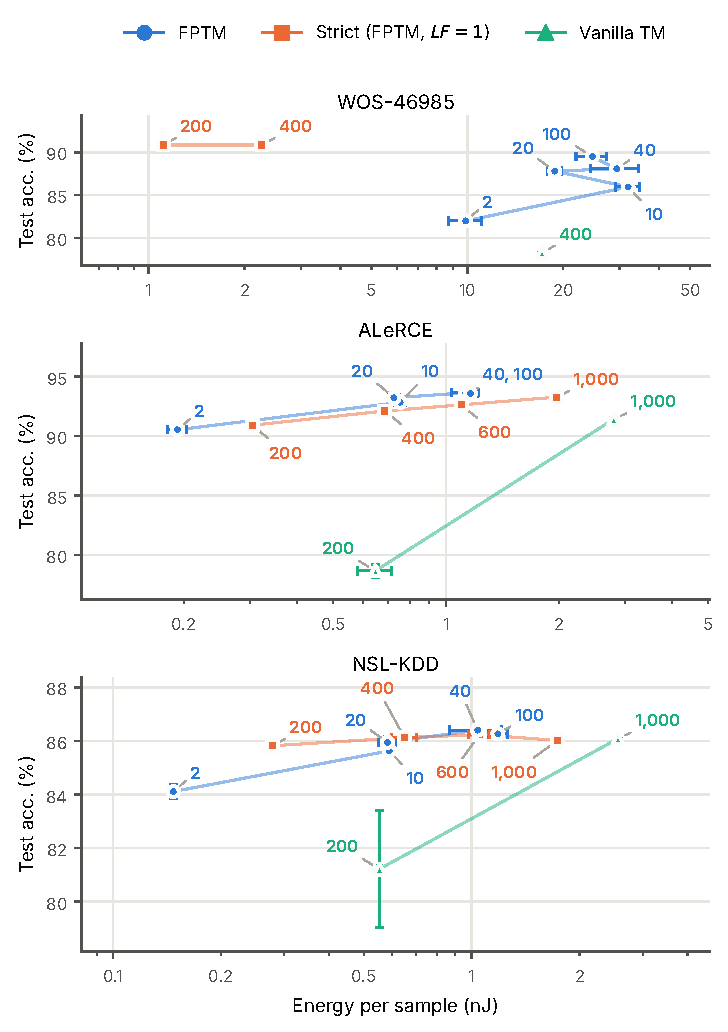
\includegraphics[width=\textwidth,height=0.78\textheight,keepaspectratio]{figures/acc_vs_energy_S.pdf}
\caption{Test accuracy versus 7~nm \gainp{} energy per sample in Mapping~S (optimistic corner), mean and standard deviation over seeds. Energy includes the controller, which dominates at this corner on WOS-46985, and excludes input loading and model-SRAM leakage. Labels give the clauses per class. Points without visible error bars are single-seed runs or have a standard deviation smaller than the marker. Some markers overlap. Overlapping markers of the same family share one label, such as ``40, 100'' on ALeRCE. The axis ranges differ between panels.}
\label{fig:paretofull}
\end{figure}

\section{Mapping C results}\label{mapCres}
Table~\ref{tab:mapC} gives the full Mapping~C results of the accuracy-oriented models. Section~5.4 of the main text summarizes them.

\begin{sidewaystable}
\footnotesize
\setlength{\tabcolsep}{4pt}
\centering
\caption{Mapping~C (clause-stationary) at the 7~nm corners, mean over seeds. Energy includes the controller (M6). The cross-column vote reduction is excluded. Its operation count equals the number of clause columns. Area at the 7~nm cell size. Latency includes refresh.}
\label{tab:mapC}
\begin{tabular}{lrrrrrrrrr}
\toprule
\multirow{2}{*}{Model (cl./class)} & Used & Clause & Sub- & Area & Cycles & \multicolumn{2}{c}{Latency ($\mu$s)} & \multicolumn{2}{c}{Energy (nJ/sample)} \\
 & features & columns & arrays & (mm$^2$) & & cons. & opt. & cons. & opt. \\
\midrule
\multicolumn{10}{l}{\textit{WOS-46985}} \\
FPTM (2) & 7,859 & 14 & 62 & \hyp{0.0452} & 768,881 & \hyp{1,155} & \hyp{776} & \hyp{3,612} & \hyp{1,485} \\
FPTM (10) & 9,399 & 70 & 148 & \hyp{0.108} & 469,717 & \hyp{706} & \hyp{474} & \hyp{2,990} & \hyp{1,032} \\
FPTM (20) & 9,090 & 140 & 215 & \hyp{0.157} & 236,316 & \hyp{355} & \hyp{239} & \hyp{1,866} & \hyp{573} \\
FPTM (40) & 9,379 & 280 & 370 & \hyp{0.270} & 243,830 & \hyp{366} & \hyp{246} & \hyp{2,746} & \hyp{716} \\
FPTM (100) & 9,432 & 700 & 818 & \hyp{0.596} & 132,079 & \hyp{198} & \hyp{133} & \hyp{2,753} & \hyp{582} \\
Strict (200) & 8,930 & 1,400 & 1,540 & \hyp{1.12} & 3 & \hyp{0.00451} & \hyp{0.00303} & \hyp{96.4} & \hyp{9.51} \\
Strict (400) & 9,628 & 2,800 & 3,344 & \hyp{2.44} & 3 & \hyp{0.00451} & \hyp{0.00303} & \hyp{208} & \hyp{20.5} \\
Vanilla TM (400) & 9,993 & 2,798 & 3,476 & \hyp{2.53} & 3 & \hyp{0.00451} & \hyp{0.00303} & \hyp{216} & \hyp{21.3} \\
\midrule
\multicolumn{10}{l}{\textit{ALeRCE}} \\
FPTM (2) & 944 & 30 & 8 & \hyp{0.00607} & 91,244 & \hyp{137} & \hyp{92.1} & \hyp{380} & \hyp{166} \\
FPTM (10) & 1,161 & 150 & 30 & \hyp{0.0219} & 57,800 & \hyp{86.9} & \hyp{58.4} & \hyp{326} & \hyp{115} \\
FPTM (20) & 1,164 & 300 & 50 & \hyp{0.0364} & 30,258 & \hyp{45.5} & \hyp{30.6} & \hyp{222} & \hyp{65.9} \\
FPTM (40) & 1,172 & 600 & 100 & \hyp{0.0729} & 30,457 & \hyp{45.8} & \hyp{30.8} & \hyp{332} & \hyp{78.9} \\
FPTM (100) & 1,172 & 1,500 & 240 & \hyp{0.175} & 16,434 & \hyp{24.7} & \hyp{16.6} & \hyp{343} & \hyp{61.4} \\
Strict (200) & 1,172 & 3,000 & 470 & \hyp{0.343} & 3 & \hyp{0.00451} & \hyp{0.00303} & \hyp{27.2} & \hyp{2.68} \\
Strict (400) & 1,172 & 6,000 & 940 & \hyp{0.685} & 3 & \hyp{0.00451} & \hyp{0.00303} & \hyp{54.3} & \hyp{5.36} \\
Strict (600) & 1,172 & 9,000 & 1,410 & \hyp{1.03} & 3 & \hyp{0.00451} & \hyp{0.00303} & \hyp{81.5} & \hyp{8.04} \\
Strict (1,000) & 1,172 & 15,000 & 2,350 & \hyp{1.71} & 3 & \hyp{0.00451} & \hyp{0.00303} & \hyp{136} & \hyp{13.4} \\
Vanilla TM (200) & 1,168 & 2,995 & 470 & \hyp{0.343} & 3 & \hyp{0.00451} & \hyp{0.00303} & \hyp{27.0} & \hyp{2.67} \\
Vanilla TM (1,000) & 1,172 & 14,964 & 2,340 & \hyp{1.71} & 3 & \hyp{0.00451} & \hyp{0.00303} & \hyp{135} & \hyp{13.4} \\
\midrule
\multicolumn{10}{l}{\textit{NSL-KDD}} \\
FPTM (2) & 178 & 46 & 2 & \hyp{0.00146} & 16,143 & \hyp{24.3} & \hyp{16.3} & \hyp{68.6} & \hyp{29.3} \\
FPTM (10) & 178 & 229 & 8 & \hyp{0.00583} & 8,650 & \hyp{13.0} & \hyp{8.73} & \hyp{53.3} & \hyp{17.4} \\
FPTM (20) & 178 & 458 & 16 & \hyp{0.0117} & 4,613 & \hyp{6.93} & \hyp{4.66} & \hyp{39.1} & \hyp{10.4} \\
FPTM (40) & 178 & 913 & 30 & \hyp{0.0219} & 4,613 & \hyp{6.93} & \hyp{4.66} & \hyp{60.5} & \hyp{12.6} \\
FPTM (100) & 178 & 2,300 & 72 & \hyp{0.0525} & 2,518 & \hyp{3.78} & \hyp{2.54} & \hyp{66.3} & \hyp{10.3} \\
Strict (200) & 178 & 4,599 & 144 & \hyp{0.105} & 3 & \hyp{0.00451} & \hyp{0.00303} & \hyp{6.39} & \hyp{0.635} \\
Strict (400) & 178 & 9,196 & 288 & \hyp{0.210} & 3 & \hyp{0.00451} & \hyp{0.00303} & \hyp{12.8} & \hyp{1.26} \\
Strict (600) & 178 & 13,797 & 432 & \hyp{0.315} & 3 & \hyp{0.00451} & \hyp{0.00303} & \hyp{19.2} & \hyp{1.89} \\
Strict (1,000) & 178 & 22,986 & 720 & \hyp{0.525} & 3 & \hyp{0.00451} & \hyp{0.00303} & \hyp{31.9} & \hyp{3.15} \\
Vanilla TM (200) & 178 & 4,597 & 144 & \hyp{0.105} & 3 & \hyp{0.00451} & \hyp{0.00303} & \hyp{6.39} & \hyp{0.635} \\
Vanilla TM (1,000) & 178 & 22,966 & 718 & \hyp{0.523} & 3 & \hyp{0.00451} & \hyp{0.00303} & \hyp{31.9} & \hyp{3.15} \\
\bottomrule
\end{tabular}

\end{sidewaystable}

\section{CPU inference}\label{cpu}
We ran every exported model on one core of an Intel Xeon processor at 2.10~GHz. Table~\ref{tab:cpu} lists the inference times.

\begin{table}[H]
\footnotesize
\setlength{\tabcolsep}{4pt}
\centering
\caption{CPU inference time with the fastest single-thread kernel, as mean $\pm$ standard deviation over seeds, which includes timing noise. \gainp{} energy per sample in Mapping~S at the conservative corner, including the controller and input loading and excluding model-SRAM leakage (M7). CPU energy is a lower bound that assumes a core power of 1~W. Ratio: CPU energy bound over \gainp{} energy.}
\label{tab:cpu}
\begin{tabular}{lrlrrr}
\toprule
\multirow{2}{*}{Model (cl./class)} & CPU time & CPU & CPU energy & \gainp{} energy & \multirow{2}{*}{Ratio} \\
 & ($\mu$s/sample) & kernel & at 1~W ($\mu$J) & (nJ, cons.) & \\
\midrule
\multicolumn{6}{l}{\textit{WOS-46985}} \\
FPTM (2) & 3.95 $\pm$ 0.10 & dense & \hyp{3.95} & \hyp{35.4} & \hyp{111} \\
FPTM (10) & 7.17 $\pm$ 0.21 & dense & \hyp{7.17} & \hyp{113} & \hyp{63.6} \\
FPTM (20) & 10.72 $\pm$ 0.33 & dense & \hyp{10.7} & \hyp{64.8} & \hyp{165} \\
FPTM (40) & 17.46 $\pm$ 0.27 & dense & \hyp{17.5} & \hyp{101} & \hyp{173} \\
FPTM (100) & 37.83 $\pm$ 1.11 & dense & \hyp{37.8} & \hyp{84.1} & \hyp{450} \\
Strict (200) & 29.51 $\pm$ 2.19 & sliced & \hyp{29.5} & \hyp{4.15} & \hyp{7,110} \\
Strict (400) & 33.22 $\pm$ 3.06 & sliced & \hyp{33.2} & \hyp{8.12} & \hyp{4,090} \\
Vanilla TM (400) & 97.95 & sliced & \hyp{98.0} & \hyp{56.7} & \hyp{1,727} \\
\midrule
\multicolumn{6}{l}{\textit{ALeRCE}} \\
FPTM (2) & 0.45 $\pm$ 0.01 & dense & \hyp{0.447} & \hyp{1.20} & \hyp{373} \\
FPTM (10) & 1.83 $\pm$ 0.04 & dense & \hyp{1.83} & \hyp{4.66} & \hyp{393} \\
FPTM (20) & 3.61 $\pm$ 0.05 & dense & \hyp{3.61} & \hyp{4.44} & \hyp{813} \\
FPTM (40) & 6.94 $\pm$ 0.19 & dense & \hyp{6.94} & \hyp{6.85} & \hyp{1,013} \\
FPTM (100) & 15.50 $\pm$ 0.30 & sliced & \hyp{15.5} & \hyp{6.75} & \hyp{2,297} \\
Strict (200) & 5.73 $\pm$ 0.05 & sliced & \hyp{5.73} & \hyp{1.91} & \hyp{2,999} \\
Strict (400) & 7.98 $\pm$ 0.11 & sliced & \hyp{7.98} & \hyp{4.29} & \hyp{1,859} \\
Strict (600) & 10.01 $\pm$ 0.14 & sliced & \hyp{10.0} & \hyp{6.85} & \hyp{1,461} \\
Strict (1,000) & 14.46 & sliced & \hyp{14.5} & \hyp{12.3} & \hyp{1,178} \\
Vanilla TM (200) & 10.76 $\pm$ 1.00 & sliced & \hyp{10.8} & \hyp{4.24} & \hyp{2,536} \\
Vanilla TM (1,000) & 27.25 & sliced & \hyp{27.2} & \hyp{17.9} & \hyp{1,521} \\
\midrule
\multicolumn{6}{l}{\textit{NSL-KDD}} \\
FPTM (2) & 0.21 $\pm$ 0.00 & dense & \hyp{0.211} & \hyp{1.29} & \hyp{163} \\
FPTM (10) & 0.87 $\pm$ 0.01 & dense & \hyp{0.875} & \hyp{5.15} & \hyp{170} \\
FPTM (20) & 1.88 $\pm$ 0.03 & dense & \hyp{1.88} & \hyp{5.05} & \hyp{373} \\
FPTM (40) & 4.32 $\pm$ 0.15 & dense & \hyp{4.32} & \hyp{8.96} & \hyp{483} \\
FPTM (100) & 12.01 $\pm$ 0.04 & dense & \hyp{12.0} & \hyp{10.0} & \hyp{1,197} \\
Strict (200) & 3.88 $\pm$ 0.10 & sliced & \hyp{3.88} & \hyp{2.46} & \hyp{1,578} \\
Strict (400) & 7.12 $\pm$ 0.11 & sliced & \hyp{7.12} & \hyp{5.74} & \hyp{1,242} \\
Strict (600) & 10.29 $\pm$ 0.19 & sliced & \hyp{10.3} & \hyp{9.28} & \hyp{1,109} \\
Strict (1,000) & 15.69 & sliced & \hyp{15.7} & \hyp{15.3} & \hyp{1,026} \\
Vanilla TM (200) & 8.30 $\pm$ 0.37 & sliced & \hyp{8.30} & \hyp{4.97} & \hyp{1,669} \\
Vanilla TM (1,000) & 30.38 & sliced & \hyp{30.4} & \hyp{22.8} & \hyp{1,332} \\
\bottomrule
\end{tabular}

\end{table}

\hyp{We bound the CPU energy from below by assuming that the active core draws at least 1~W. For this comparison, the \gainp{} energy includes input loading (M4), because the CPU time includes input packing. It excludes model-SRAM leakage (M7). Under this bound, the CPU needs between $63\times$ and about $7{,}100\times$ more energy per classification than the \gainp{} at the conservative corner, for every model (Table~\ref{tab:cpu}). For the 20-clause ALeRCE FPTM, the ratio is about $810\times$. Equivalently, at equal power, \gainp{} would classify $63\times$ to about $7{,}100\times$ more samples per second.}

\textit{Kernels and timing protocol.} We implemented three single-threaded Numba kernels.
The dense kernel packs the input into 64-bit words and counts the failing literals of a clause with population counts.
The sparse kernel walks the literal list of each clause and stops once the clause score is zero.
The bit-sliced kernel packs 64 samples into each 64-bit word. For strict and vanilla models, it ANDs the literal words of a clause and stops when no sample remains. For FPTM models, it keeps a vertical binary miss counter per clause.
Every kernel reproduced the software reference on every test sample of all 80 runs.
Every kernel within $1.5\times$ of the fastest pilot run was timed as the median of five repetitions over the full test set, each lasting at least 0.5~s. The timing includes input packing. We ran two independent passes over all runs and report, for each run, the fastest kernel of the faster pass.
The dense kernel was the fastest for all FPTM runs except the three runs of the 100-clause ALeRCE model, and the bit-sliced kernel for all strict and vanilla runs.
Both passes ran on the same processor. The two passes differed by up to 33\% for the same run, relative to the faster pass, with a median of 4.4\%. The standard deviations in Table~\ref{tab:cpu} therefore include timing noise.

\section{Sensitivity analysis}\label{sens}
We test how the accuracy-oriented ALeRCE comparison, the 20-clause FPTM against the 600-clause $\LF=1$ model, depends on the modelling choices.
At the 16~nm reference points, the strict model needs \hyp{1.51$\times$} (system point) and \hyp{1.54$\times$} (circuit point) the energy of the FPTM model.
At the 7~nm corners the ratio is \hyp{1.55$\times$} (conservative) and \hyp{1.51$\times$} (optimistic).
If every cycle is charged one cell operation per column, regardless of the number of unmasked rows, the ratio becomes \hyp{1.28$\times$} at the conservative corner.
The ranking therefore holds for both energy models tested.
The controller share of the Mapping~S energy is \hyp{3\% to 4\%} on NSL-KDD, \hyp{14\% to 17\%} on ALeRCE and \hyp{41\% to 54\%} on WOS-46985 at the conservative corner. At the optimistic corner it is \hyp{13\% to 17\%}, \hyp{41\% to 45\%} and \hyp{69\% to 84\%}, because the array energy shrinks more than the upper-estimate controller energy. Without the controller, the strict-to-FPTM energy ratio on ALeRCE is \hyp{1.55$\times$}. With a five times lower sequencer and model-read energy, it is \hyp{1.55$\times$}, and with a 64-subarray macro it is \hyp{1.53$\times$}.
With a $10\times$ shorter retention time, the refresh overhead of the FPTM batch latency rises from \hyp{1.4\%} to \hyp{14.3\%} at the conservative corner. Its energy per sample rises from \hyp{4.42~nJ} to \hyp{5.90~nJ}.
Static energy is a large share wherever logical columns are tall and programs are long. For the 100-clause WOS-46985 FPTM it is \hyp{25\%} of the energy at the conservative corner, against \hyp{13\%} for the 200-clause $\LF=1$ model.
The refresh model assumes that the subarrays of a logical column refresh in lockstep through their local sense amplifiers (Section~\ref{modelling}). If refresh instead used the shared sense amplifier, the $h$ subarrays would be refreshed one after another, and each refresh would stall the array for $h\times512$ cycles. This stall would take \hyp{14.3\%} (conservative) and \hyp{9.7\%} (optimistic) of every refresh period on ALeRCE ($h=10$), and \hyp{2.9\%} and \hyp{1.9\%} on NSL-KDD ($h=2$). On WOS-46985 ($h=79$) it would take \hyp{113\%} and \hyp{76\%} of the period, so Mapping~S would not be feasible at the conservative corner. Mapping~C on WOS-46985 stacks up to 79 subarrays and would be affected in the same way. All ALeRCE models use the same $h$ in Mapping~S, so their ranking would not change.

\section{Mapping S cycle count versus model size}\label{spearman}
For each dataset, Table~\ref{tab:spearman} relates the Mapping~S cycle count of the 11 FPTM configurations (five accuracy-oriented and six energy-oriented) to three measures of model size.
The measures are the clause count per class, the number of included literals per class, and this number weighted by $\log_2(\LF+1)$, which approximates the width of the miss counter.
The weighting is a descriptive choice made after the experiments.
The cycle count follows the weighted literal count closely (Spearman rank correlation 0.92 to 0.99) and the clause count only weakly (0.31 to 0.65).

\begin{table}[H]
\centering
\caption{Spearman rank correlation between the Mapping~S cycle count and model size, per dataset, over the FPTM configurations of both hyperparameter sets.}
\label{tab:spearman}
\begin{tabular}{lrrrr}
\toprule
Dataset & Config. & Clauses & Literals & Lit.\ $\times\log_2(\LF+1)$ \\
\midrule
WOS-46985 & 11 & 0.31 & 0.57 & 0.92 \\
ALeRCE & 11 & 0.53 & 0.86 & 0.99 \\
NSL-KDD & 11 & 0.65 & 0.93 & 0.96 \\
\bottomrule
\end{tabular}
\end{table}

\section{Additional discussion}\label{discussion}
\textit{Strict models from the FPTM trainer.} At equal clause count, the strict models trained with the FPTM trainer are more accurate than the vanilla TM.
The only exception is NSL-KDD with 1,000 clauses per class, where the two test accuracies differ by less than 0.1 points (Table~4 of the main text).
They differ from the vanilla baseline in several trainer details and hyperparameters (Sections~2.2 and~4.2 of the main text), so we do not attribute the gap to one cause.
For \gainp{}, these strict models are attractive because each of their clauses costs one COMPARE {cycle} in Mapping~S.

\textit{Mapping choice.} Mapping~S amortizes the program over all columns. It suits batch inference. Its latency does not depend on the batch size. \hyp{Its energy per sample is lowest when the batch fills the macro.}
Mapping~C writes the model once and leaves the input on the searchlines. It processes one sample at a time. For strict models, it needs only 3 array cycles per sample. However, strict models need large arrays and an external reduction of thousands of clause outputs.
FPTM shrinks both. On ALeRCE, the accuracy-oriented 20-clause FPTM needs about $47\times$ less array area and $50\times$ fewer reduction operations than the 1,000-clause $\LF=1$ model. The price is about 30,000 cycles per sample {and, before the external reduction, \hyp{$1.6\times$ to $4.9\times$} more energy per sample}.
For FPTM and strict models, Mapping~C also costs more energy per sample than Mapping~S. Every sample activates the whole model array, and the controller energy is not shared between samples. \hyp{For FPTM models, the controller accounts for 14\% to 90\% of the Mapping~C energy at the conservative corner and 40\% to 97\% at the optimistic corner. Without the controller, Mapping~C still costs more than Mapping~S for every FPTM and strict model.}


\end{document}
